\chapter{A/D Conversion}

\usetikzlibrary{shapes,arrows}
    \usetikzlibrary{positioning}
    
\begin{figure} [H]
    \centering
    \tikzstyle{frame} = [
        rectangle, draw, 
        text width=4em, text centered,
        minimum height=4em
    ]
    \tikzstyle{line} = [draw, -latex']
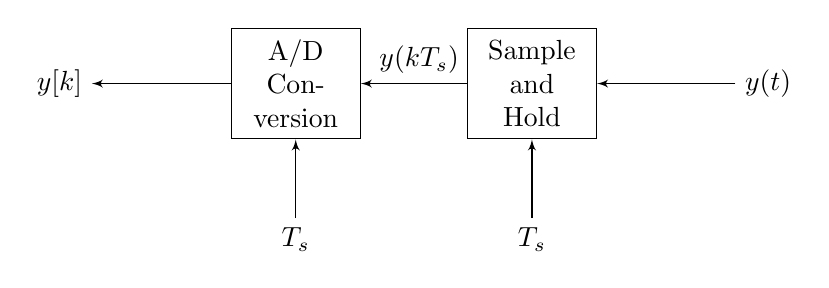
\begin{tikzpicture}[node distance = 3cm]
    \node [frame] (A/D) {A/D Conversion};
    \node [left of=A/D] (yk) {$y[k]$};
    \node [frame, right of=A/D] (SH)  {Sample and Hold};
    \node [right of=SH] (yt)  {$y(t)$};
    \node [below=1cm of SH] (ts)  {$T_s$};
    \node [below=1cm of A/D] (TS)  {$T_s$};

    \path [line] (A/D) -- (yk);
    \path [line] (SH) -- node[above,pos=.45] {$y(kT_s)$} (A/D);
    \path [line] (yt) -- (SH);
    \path [line] (ts) -- (SH);
    \path [line] (TS) -- (A/D);
\end{tikzpicture}
    \caption{A figure of the analog to digital converter....} 
    \label{fig:SH_ADC}
\end{figure}



\textbf{Midlertidig disposition}
\begin{itemize}
    \item A/D conversion
    \begin{itemize}
        \item Bits needs to be explained (kan springes lidt over)
        \item Sample and hold
    \end{itemize}
    \item Modeling the process
    \begin{itemize}
        \item Dirac Delta
        \item Unit impulse response
    \end{itemize}
    \item Sample rate (uses Fourier as example)
    \item Aliasing (DFT)
    \item Quantization
\end{itemize}

\section{Sampling}
In section ?? it was established that a continues signal y(t) can be represented as a discreet sequence y[t] of samples with a sample period $T$. 
 It is often desirable to reconstruct signal from the discreet sequence. To do so the sequence must be uniquely determined. What or not a discreet sequence is uniquely determined is dependent on two parameters, the sample period and the bandwidth of the original signal. As described in section ?? a single can decomposed into the its frequency. The bandwidth the maximum frequency of a signal. This is possible to determine since the frequency is often but on not always bounded in practice.   

\begin{theorem}{Nyquist-Shannon theorem}
    If the denotes $\omega_N$ the maximum frequency  of a signal $y(t)$ then in order for the samples $y[k]$ to be uniquely determined the sample frequency $\omega_s$ must satisfy
    \begin{align*}
        \omega_s \geq 2\omega_N.
    \end{align*}
\end{theorem}
